\chapter{Слабые поля, гравитационные волны и принцип действия}

Точные уравнения общей теории относительности нелинейны, и их запись по компонентам может стать устрашающе громоздкой еще до того, как будет решена хотя бы одна физическая задача. Для последней лекции курса лучше отделить принципиальные вопросы от технических выкладок. Мы спросим, во что превращаются уравнения Эйнштейна, когда гравитационное поле слабо, выделим волны, содержащиеся в этом приближении, а затем закончим тем, что увидим, как полные уравнения поля укладываются в удивительно компактный принцип действия.

Обсуждение организуют три вопроса. Что означает слабое гравитационное поле? Почему слабая теория линейна, хотя точная теория таковой не является? И какие физические эффекты отличают гравитационную волну от простой волнистости координат?

\section{Малое возмущение равновесной геометрии}

Слабость — это схема приближения. Если безразмерное возмущение имеет величину \(\epsilon\ll1\), то его квадрат имеет величину \(\epsilon^2\), и в расчете первого порядка последовательно отбрасывают последний. Знакомый пример — механическая система, совершающая малые колебания около равновесия. Ее точные уравнения могут быть нелинейными, но достаточно малые колебания подчиняются линейным уравнениям.

Для гравитации равновесным фоном будет пустое плоское пространство-время. Начнем с вакуумного уравнения Эйнштейна,
\begin{equation}
 R_{\mu\nu}-\frac12 g_{\mu\nu}R=0.
 \label{eq:l10-vacuum-einstein}
\end{equation}
Взятие его следа в четырех измерениях дает
\begin{equation}
 g^{\mu\nu}
 \left(R_{\mu\nu}-\frac12 g_{\mu\nu}R\right)
 =R-2R=-R=0,
\end{equation}
так что вакуумное уравнение эквивалентно
\begin{equation}
 R_{\mu\nu}=0.
 \label{eq:l10-ricci-flat}
\end{equation}

\begin{figure}[htbp]
\centering
\includegraphics[width=0.68\textwidth]{lecture_10_figure_02.png}
\caption{Вакуумное уравнение \(R_{\mu\nu}=0\), выделенное в начале рассуждения о слабом поле.}
\lectureframe{00:03:11}
\end{figure}

Здесь под равновесием понимается решение без источников и без зависимости от времени. Плоское пространство-время — простейшее такое решение. Одно уточнение существенно: плоскостность не означает, что компоненты метрики равны некоторой определенной матрице в любой системе координат. Это означает, что можно выбрать инерциальные координаты, в которых
\begin{equation}
 g_{\mu\nu}=\eta_{\mu\nu}.
\end{equation}
Это различие между геометрией и координатами, используемыми для ее описания, вскоре станет центральной тонкостью.

Теперь представим себе бурный источник, например компактную двойную систему. Вблизи поле может быть сильным, но далеко от источника возмущение распространяется и становится малым. Тогда в подходящей системе координат метрику можно записать в виде
\begin{equation}
 g_{\mu\nu}(x)=\eta_{\mu\nu}+h_{\mu\nu}(x),
 \qquad |h_{\mu\nu}|\ll1.
 \label{eq:weak-split}
\end{equation}
Возмущение \(h_{\mu\nu}\) может зависеть от всех четырех координат пространства-времени. Слабость означает, что степенями выше первой будут пренебрегать.

\section{Что сохраняется в первом порядке}

Полный тензор Риччи на этой стадии слишком громоздок, чтобы быть полезным. Достаточно его структуры. Символы Кристоффеля содержат обратную метрику и одну производную от метрики, тогда как кривизна содержит производную от символа Кристоффеля и произведение двух символов Кристоффеля:
\begin{equation}
 \Gamma\sim\frac12 g^{-1}\partial g,
 \qquad
 R\sim\partial\Gamma+\Gamma\Gamma.
 \label{eq:curvature-skeleton}
\end{equation}

\begin{figure}[htbp]
\centering
\includegraphics[width=0.84\textwidth]{lecture_10_figure_03.png}
\caption{Разложение по слабому полю и схематическое построение \(R\sim\partial\Gamma+\Gamma\Gamma\). Обозначения выявляют порядки по \(h\) без явного выписывания всех индексов.}
\lectureframe{00:10:17}
\end{figure}

Обратная метрика следует из условия
\(g^{\mu\alpha}g_{\alpha\nu}=\delta^\mu{}_\nu\). В первом порядке
\begin{equation}
 g^{\mu\nu}=\eta^{\mu\nu}-h^{\mu\nu}+O(h^2),
 \label{eq:inverse-weak}
\end{equation}
где индексы у \(h\) поднимаются фоновой метрикой. В инерциальных координатах фон постоянен,
\begin{equation}
 \partial_\alpha\eta_{\mu\nu}=0,
\end{equation}
и потому
\begin{equation}
 \partial_\alpha g_{\mu\nu}
 =\partial_\alpha h_{\mu\nu}.
\end{equation}
Следовательно,
\begin{equation}
\begin{aligned}
 \Gamma&=O(\partial h),\\
 R_{\mu\nu}
 &=O(\partial\partial h)+O\bigl((\partial h)^2\bigr)\\
 &\quad+O(h\,\partial\partial h).
\end{aligned}
 \label{eq:ricci-orders}
\end{equation}

\begin{figure}[htbp]
\centering
\includegraphics[width=0.84\textwidth]{lecture_10_figure_04.png}
\caption{Разложение обратной метрики на доске и замечание о том, что \(\partial\eta=0\). В ведущем порядке остаются только производные от \(h_{\mu\nu}\).}
\lectureframe{00:11:55}
\end{figure}

Последние два члена в уравнении~\eqref{eq:ricci-orders} квадратичны по возмущению и поэтому опускаются. Следовательно, вакуумные уравнения сводятся к линейным уравнениям, содержащим вторые производные от \(h_{\mu\nu}\). В этом и состоит весь смысл линеаризации. Это не утверждение о том, что точная теория Эйнштейна линейна.

\begin{classroomqa}
\audiencequestion{Тензор кривизны имеет четыре индекса, тогда как тензор Риччи — два. Если две производные уже несут индексы, а \(h_{\mu\nu}\) несет еще два, то как тогда получается правильное число индексов?}
\lecturerresponse{Тензор Риччи получается сверткой по паре индексов тензора кривизны. Метрика, используемая при этой свертке, оставляет два свободных индекса — как раз ту пару, которую несет \(R_{\mu\nu}\). Символическая запись \(\partial\partial h\) опускает эти свертки; это подсчет порядков, а не полная формула с индексами.
\lecturetimestamp{00:18:45--00:19:53}}
\end{classroomqa}

\begin{classroomqa}
\audiencequestion{Появляются ли при свертке с обратной метрикой члены типа \(h\,\partial^2h\) и, если да, почему ими можно пренебречь?}
\lecturerresponse{Появляются. Замена \(g^{-1}\) на \(\eta^{-1}-h+\cdots\) порождает как линейный член \(\eta^{-1}\partial^2h\), так и поправки, содержащие второе \(h\). Последние квадратичны. По тому же правилу отбрасываются \(h\,\partial h\), \(h\,\partial^2h\) и \((\partial h)^2\). Сохранять только одну степень возмущения — это и есть именно то приближение, которое здесь делается.
\lecturetimestamp{00:19:55--00:21:14}}
\end{classroomqa}

\section{Почему уравнения имеют волновой вид}

Полевые уравнения со вторыми производными естественно наводят на мысль о волновом распространении. Для скалярной функции, распространяющейся вдоль оси \(z\), прототипом служит
\begin{equation}
 \left(\partial_t^2-\partial_z^2\right)\phi=0,
\end{equation}
решения которого включают произвольные профили, бегущие вправо и влево,
\begin{equation}
 \phi(z,t)=f(z-t)+g(z+t).
\end{equation}
В трех пространственных измерениях то же уравнение имеет вид
\begin{equation}
 \left(\partial_t^2-\nabla^2\right)\phi=0.
\end{equation}
Его линейность допускает суперпозицию: сумма двух решений также является решением.

Гравитация не является скалярным полем. Возмущение имеет тензорные компоненты, и уравнение \(R_{\mu\nu}=0\) поначалу как будто задает много уравнений для компонент. Не все они независимы; часть из них — связи, а часть отражает свободу выбора координат. Аналогия здесь — теория Максвелла, где совокупность полевых уравнений в конечном счете оставляет только физические поперечные волны.

После наложения подходящих координатных условий излучательные компоненты подчиняются обычному волновому уравнению,
\begin{equation}
 \Box h_{\mu\nu}=0,
 \qquad
 \Box=\eta^{\alpha\beta}\partial_\alpha\partial_\beta.
 \label{eq:linear-wave}
\end{equation}
Точные знаки внутри \(\Box\) зависят от соглашения о сигнатуре; его содержание от этого не меняется. Возмущения распространяются по световому конусу.

\section{Волнистость координат — не гравитационные волны}

Прежде чем признать всякое решение линеаризованных уравнений физической волной, нужно вернуться к оговорке о координатах. Плоское пространство можно описать искривленными координатными линиями. Тогда компоненты его метрики отличаются от своих декартовых значений, хотя его кривизна по-прежнему равна нулю.

Пример дает сама доска. Проведем на ее плоской поверхности прямые декартовы координаты и запишем
\begin{equation}
 ds^2=\delta_{mn}\,dx'^m dx'^n.
\end{equation}
Теперь переобозначим те же точки слегка волнистыми координатами,
\begin{equation}
 x'^m=x^m+f^m(x).
 \label{eq:small-coordinate-change}
\end{equation}
Дифференциалы принимают вид
\begin{equation}
 dx'^m=dx^m+\partial_n f^m\,dx^n.
\end{equation}
Подставляя это в линейный элемент и сохраняя только первый порядок по \(f\), получаем
\begin{align}
 ds^2
 &=\delta_{mn}dx^m dx^n\\
 &\quad+\left(\partial_m f_n+\partial_n f_m\right)dx^m dx^n
 +O(f^2).
\end{align}
Итак, кажущееся возмущение вида
\begin{equation}
 h_{mn}=\partial_m f_n+\partial_n f_m
 \label{eq:pure-gauge}
\end{equation}
может вообще не описывать никакой новой геометрии. Это плоское пространство в волнистых координатах.

\begin{figure}[htbp]
\centering
\includegraphics[width=0.84\textwidth]{lecture_10_figure_05.png}
\caption{Вычисление для волнистых координат на доске. Малое преобразование координат индуцирует малое на вид \(h_{mn}\), хотя сама доска остается плоской.}
\lectureframe{00:27:54}
\end{figure}

Уравнение~\eqref{eq:pure-gauge} есть линеаризованная форма координатной, или калибровочной, свободы. Чтобы исключить эти фиктивные возмущения, нужны дополнительные условия. Подробная калибровочная алгебра здесь не разрабатывается. Важна ее роль: она устраняет изменения описания, сохраняя изменения кривизны. После учета свободы координат и уравнений-связей физическое содержание сводится к двум независимым поляризациям волны.

\begin{figure}[htbp]
\centering
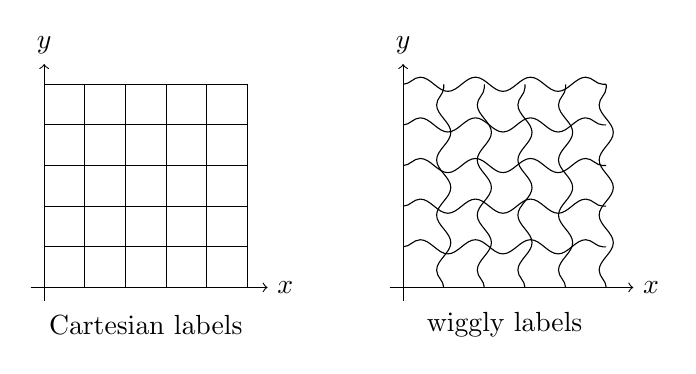
\begin{tikzpicture}[scale=0.86]
\begin{scope}
\draw[->] (-0.2,0) -- (3.3,0) node[right] {$x$};
\draw[->] (0,-0.2) -- (0,3.3) node[above] {$y$};
\foreach \u in {0.6,1.2,1.8,2.4,3.0}{
  \draw (\u,0) -- (\u,3.0);
  \draw (0,\u) -- (3.0,\u);
}
\node at (1.5,-0.55) {Cartesian labels};
\end{scope}
\begin{scope}[xshift=5.3cm]
\draw[->] (-0.2,0) -- (3.4,0) node[right] {$x$};
\draw[->] (0,-0.2) -- (0,3.3) node[above] {$y$};
\foreach \u in {0.6,1.2,1.8,2.4,3.0}{
  \draw[decorate,decoration={snake,amplitude=0.09cm,segment length=0.7cm}]
    (\u,0) -- (\u,3.0);
  \draw[decorate,decoration={snake,amplitude=0.09cm,segment length=0.7cm}]
    (0,\u) -- (3.0,\u);
}
\node at (1.5,-0.55) {wiggly labels};
\end{scope}
\end{tikzpicture}
\caption{Геометрия остается плоской, тогда как координатная сетка меняется. Одни только компоненты метрики не могут решить, является ли возмущение физическим.}
\end{figure}

\section{Волна, распространяющаяся вдоль оси z}

Выберем плоскую волну, распространяющуюся в положительном направлении \(z\). Ее фазу можно записать как
\begin{equation}
 k(z-t),
\end{equation}
так что типичная компонента имеет вид
\begin{equation}
 h_{\mu\nu}(z,t)
 =h_{\mu\nu}^{(0)}\sin k(z-t).
 \label{eq:plane-wave}
\end{equation}
Поверхности постоянной фазы удовлетворяют условию \(z-t=\text{constant}\); следовательно, скорость распространения равна скорости света.

В поперечно-бесследовом описании компоненты, содержащие временной индекс или \(z\)-индекс, обращаются в нуль:
\begin{equation}
 h_{0\mu}=0,
 \qquad
 h_{z\mu}=0.
 \label{eq:tt-transverse}
\end{equation}
Остается только блок \(x\)-\(y\). Он симметричен и бесследов,
\begin{equation}
 h_{xy}=h_{yx},
 \qquad
 h_{xx}+h_{yy}=0.
 \label{eq:tt-trace}
\end{equation}

\begin{figure}[htbp]
\centering
\includegraphics[width=0.84\textwidth]{lecture_10_figure_06.png}
\caption{Волна, распространяющаяся вдоль \(z\), изображенная как стопка поперечных плоскостей. Сохраняющиеся амплитуды \(x\)-\(y\) подчиняются условию \(h_{xx}+h_{yy}=0\).}
\lectureframe{00:43:36}
\end{figure}

Следовательно, имеются две независимые структуры. Для \(i,j\in\{x,y\}\) их можно записать как
\begin{equation}
 h^{\mathrm{TT}}_{ij}(z,t)
 =
 \begin{pmatrix}
 h_+ & h_\times\\
 h_\times & -h_+
 \end{pmatrix}
 \sin k(z-t).
 \label{eq:polarization-matrix}
\end{equation}
Диагональная структура называется плюсовой поляризацией. Недиагональная структура называется крестовой поляризацией. Поворот поперечных осей на \(45^\circ\) переводит одну структуру в другую, а произвольная линейно поляризованная волна является суперпозицией этих двух. В этой теории нет других независимых поляризаций.

\begin{figure}[htbp]
\centering
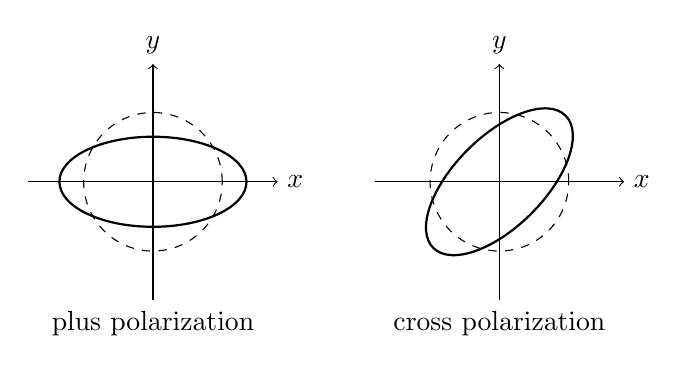
\begin{tikzpicture}[scale=0.88]
\begin{scope}
\draw[->] (-1.8,0) -- (1.8,0) node[right] {$x$};
\draw[->] (0,-1.7) -- (0,1.7) node[above] {$y$};
\draw[dashed] (0,0) circle (1.0);
\draw[thick] (0,0) ellipse (1.35 and 0.65);
\node at (0,-2.05) {plus polarization};
\end{scope}
\begin{scope}[xshift=5.0cm]
\draw[->] (-1.8,0) -- (1.8,0) node[right] {$x$};
\draw[->] (0,-1.7) -- (0,1.7) node[above] {$y$};
\draw[dashed] (0,0) circle (1.0);
\draw[thick,rotate=45] (0,0) ellipse (1.35 and 0.65);
\node at (0,-2.05) {cross polarization};
\end{scope}
\end{tikzpicture}
\caption{В течение половины периода одно поперечное направление растягивается, а перпендикулярное сжимается. Еще через половину периода деформация становится противоположной.}
\end{figure}

\section{От компонент метрики к физической деформации}

Зафиксируем \(z\) и \(t\) и рассмотрим поперечную плоскость. Для чистой волны с поляризацией «плюс»,
\begin{equation}
 ds_\perp^2
 =(1+h_{xx})\,dx^2+(1-h_{xx})\,dy^2.
 \label{eq:transverse-distance}
\end{equation}
Когда \(h_{xx}>0\), фиксированный координатный интервал в направлении \(x\) имеет немного большую собственную длину, тогда как соответствующий интервал по \(y\) имеет немного меньшую собственную длину. Полпериода спустя \(h_{xx}\) меняет знак, и роли меняются местами. Квадрат попеременно растягивается по горизонтали и сжимается по вертикали, затем сжимается по горизонтали и растягивается по вертикали. Для крестовой поляризации то же чередование происходит вдоль осей, повернутых на \(45^\circ\).

В первом порядке плечо, первоначально имеющее длину \(L\), изменяется на
\begin{equation}
 \frac{\Delta L}{L}\simeq\frac12 h_{ij}n^i n^j,
 \label{eq:fractional-strain}
\end{equation}
где \(\mathbf n\) направлен вдоль плеча. Эта формула выражает возмущение метрики через безразмерную относительную деформацию, измеряемую детектором.

\begin{classroomqa}
\audiencequestion{Метровая линейка удерживается электромагнитными силами и не просто изменяет свою длину покоя вслед за координатами. Не следует ли в этой картине вместо нее использовать свободно разнесенные пробные массы?}
\lecturerresponse{Это различие важно. Реальный стержень обладает упругостью, поэтому приливное поле возбуждает в нем напряжения; стальной и деревянный стержни, вообще говоря, будут реагировать по-разному. Свободно подвешенные пробные массы позволяют избежать именно этой упругой реакции и более непосредственно выявляют относительное ускорение. И в том и в другом случае проходящая волна не сводится просто к переименованию точек. Ее зависящая от времени кривизна производит физический эффект.
\lecturetimestamp{00:47:23--00:48:48}}
\end{classroomqa}

Точное локальное утверждение дается уравнением геодезического отклонения. Для близких свободно падающих частиц, разделенных вектором \(\xi^i\),
\begin{equation}
 \frac{d^2\xi^i}{dt^2}
 =-R^i{}_{0j0}\,\xi^j.
 \label{eq:geodesic-deviation}
\end{equation}
В слабой поперечно-бесследовой волне,
\begin{equation}
 R_{0i0j}=-\frac12\ddot h^{\mathrm{TT}}_{ij},
 \label{eq:tidal-curvature}
\end{equation}
так что осциллирующая метрика порождает знакопеременное приливное ускорение. Именно поэтому волну, зависящую от времени, нельзя считать просто статическим выбором линеек. У нее ненулевая кривизна.

\begin{classroomqa}
\audiencequestion{Чем можно измерить сжатие и растяжение, если затронута каждая линейка в этой области?}
\lecturerresponse{Тензодатчик может зарегистрировать подлинное напряжение, наведенное в материальном теле. Еще лучше отслеживать меняющееся расстояние между свободно подвешенными массами. Статическое однородное масштабирование могло бы быть поглощено измерительным прибором, но осциллирующая кривизна вызывает отклик, который можно зарегистрировать.
\lecturetimestamp{00:51:10--00:52:02}}
\end{classroomqa}

\section{Источники и детекторы}

Электромагнитные волны порождаются движущимися зарядами и токами. Гравитационные волны порождаются движущимися распределениями массы и энергии. Сохранение энергии и импульса исключает гравитационное монопольное и дипольное излучение для изолированной системы, поэтому ведущим излучающим мультипольным моментом является квадрупольный момент. Компактная двойная система как раз дает требуемый меняющийся квадруполь: два плотных тела обращаются друг вокруг друга и излучают волны в дальнюю зону.

Вблизи двойной системы пространство-время сильно искривлено, и линейное разложение, использованное в уравнении~\eqref{eq:weak-split}, ненадежно. Далеко от нее исходящая волна распространяется по большей площади, ее амплитуда становится малой, и линеаризованное описание становится точным. Для наблюдателя на оси \(z\) относительно источника измеряемое растяжение проявляется в поперечной плоскости \(x\)-\(y\).

\begin{classroomqa}
\audiencequestion{Является ли линейка на рисунке абстрактной координатной линейкой или физической метровой линейкой, и как линейка с меняющейся длиной могла бы измерить этот эффект?}
\lecturerresponse{Это может быть физический объект, но тогда важны свойства его материала. Кривизна создает приливное напряжение; сталь и дерево не обязаны деформироваться под его действием одинаково. Сравнение их откликов уже само по себе является измерением. Более чистый детектор заменяет стержни разнесенными пробными массами и измеряет их дифференциальное движение.
\lecturetimestamp{00:54:00--00:55:19}}
\end{classroomqa}

Резонансный детектор — одна из стратегий. Если механическая система имеет собственную частоту, близкую к частоте приходящей волны, волна возбуждает ее когерентно и усиливает отклик. Интерферометр использует другую стратегию: зеркала служат пробными массами, а лазерная интерференция сравнивает эффективные длины взаимно перпендикулярных плеч. Волна с поляризацией «плюс» удлиняет одно плечо, одновременно укорачивая другое, и именно такой дифференциальный сигнал интерферометр и предназначен обнаруживать.

\begin{classroomqa}
\audiencequestion{Может ли это служить основой детектора гравитационных волн?}
\lecturerresponse{Да. Жесткий стержень почти не меняется, тогда как свободно подвешенные концевые массы могут испытывать относительное ускорение. Можно также использовать резонанс, чтобы слабое периодическое воздействие вызывало больший отклик. Ожидаемая астрофизическая относительная деформация чрезвычайно мала, порядка \(10^{-21}\), поэтому разработка детектора — это искусство превращения этого крошечного дифференциального движения в измеримый сигнал.
\lecturetimestamp{00:55:20--00:57:10}}
\end{classroomqa}

\begin{classroomqa}
\audiencequestion{Является ли LIGO примером такого детектора?}
\lecturerresponse{Да. Его основные наблюдаемые величины задаются лазерным светом, отражающимся между зеркалами в перпендикулярных плечах. Гравитационная волна изменяет относительные оптические длины путей и, следовательно, интерференционную картину. На момент этой лекции этот прибор еще не дал прямого обнаружения; позднее эта историческая ситуация изменилась.\editorialnote{Первое прямое наблюдение, GW150914, было зарегистрировано в 2015 году и объявлено в 2016 году.}
\lecturetimestamp{00:57:16--00:58:05}}
\end{classroomqa}

\begin{classroomqa}
\audiencequestion{Какая скорость распространения следует из волнового решения?}
\lecturerresponse{Скорость света. Фаза \(k(z-t)\) смещается на одну единицу по \(z\) за одну единицу по \(t\), а линеаризованное уравнение Эйнштейна имеет ту же структуру распространения по световому конусу, что и уравнение электромагнитной волны.
\lecturetimestamp{00:58:07--00:58:16}}
\end{classroomqa}

Столкновения черных дыр и компактные двойные системы — особенно перспективные источники. Вблизи столкновения гравитационное поле резко нелинейно, и значительная часть высвобожденной энергии может уноситься в виде гравитационного излучения. К тому времени, когда сигнал достигает далекого детектора, его амплитуда уже достаточно мала, чтобы линейное волновое распространение было превосходным описанием. Тем самым гравитационное излучение открывает астрономический канал, который не обязан зависеть от испускаемого света.

\section{Двойной пульсар и косвенные свидетельства}

Излучение переносит энергию. Если двойная система излучает гравитационные волны, орбитальная энергия уменьшается, тела медленно сближаются по спирали, и орбитальный период меняется. Двойной пульсар служит часами, достаточно точными, чтобы измерить это изменение. Наблюдаемая эволюция его орбиты количественно согласуется с потерей энергии, предсказанной общей теорией относительности.

В историческом контексте этой лекции это было решающим косвенным свидетельством: ни один детектор еще не зарегистрировал волну, проходящую через Землю, но орбита теряла энергию с той скоростью, которую требует гравитационное излучение. Волны уже можно было наблюдать по тому, что они делали со своим источником.

\begin{classroomqa}
\audiencequestion{Какая частота или какой период характеризует исходную систему двойного пульсара? Это миллисекундный масштаб?}
\lecturerresponse{Миллисекундный масштаб относится к вращению пульсара, а не к орбите двух звезд. В аудитории проверяют это значение и находят орбитальный период около \(7.75\) часов. Это различие важно: гравитационное излучение отслеживает орбитальное движение двойной системы, тогда как радиопульсы дают точные часы, используемые для его прослеживания.
\lecturetimestamp{01:01:27--01:03:28}}
\end{classroomqa}

\begin{classroomqa}
\audiencequestion{Насколько велик был накопленный временной сдвиг орбиты за десятилетия наблюдений?}
\lecturerresponse{Указанный накопленный сдвиг составляет примерно тридцать секунд. Мгновенное относительное изменение ничтожно мало, но десятилетия точного хронометража импульсов делают кумулятивный эффект видимым.
\lecturetimestamp{01:03:34--01:03:54}}
\end{classroomqa}

\section{Зависимость от времени, кривизна и пределы линейности}

\begin{classroomqa}
\audiencequestion{Почему выбирают поперечную плоскость \(x\)-\(y\)? Что происходит, если вместо этого рассмотреть плоскость, включающую \(x\) и \(t\)?}
\lecturerresponse{Сама волна зависит и от \(z\), и от \(t\), но «поперечный» относится к пространственным направлениям, перпендикулярным ее пространственному направлению распространения. Для волны, движущейся вдоль \(z\), физические амплитуды метрики можно выбрать в блоке \(x\)-\(y\). Другие кажущиеся компоненты отсутствуют или являются устранимыми координатными колебаниями.
\lecturetimestamp{01:02:22--01:03:17}}
\end{classroomqa}

\begin{classroomqa}
\audiencequestion{Колеблется ли само время?}
\lecturerresponse{Нет. Волна колеблется как функция времени. При фиксированном пространственном положении компоненты \(h_{ij}(z,t)\) периодически меняются. Время — это координата, от которой зависит поле, а не объект, который в этой картине попеременно растягивается и сжимается.
\lecturetimestamp{01:04:00--01:04:18}}
\end{classroomqa}

\begin{classroomqa}
\audiencequestion{Если все \(h_{0\mu}\) равны нулю, означает ли это, что нет никакой кривизны, связанной с временным направлением?}
\lecturerresponse{Она есть. Сохранившиеся пространственные компоненты зависят от времени, а кривизна содержит их вторые производные. Поэтому производные, такие как \(\partial_t^2h_{ij}\), порождают компоненты \(R_{0i0j}\). Нулевые компоненты \(h_{\mu\nu}\) с временным индексом не означают, что зависящая от времени кривизна равна нулю.
\lecturetimestamp{01:05:15--01:06:09}}
\end{classroomqa}

Линейное волновое уравнение возникло потому, что \(h\) считалось малым, а не потому, что были устранены координатные артефакты. Это две разные операции. Фиксация калибровки выделяет физические степени свободы; линеаризация отбрасывает нелинейные взаимодействия.

\begin{classroomqa}
\audiencequestion{Уравнения Эйнштейна нелинейны, но получающееся волновое уравнение линейно. Обусловлена ли эта линейность устранением нефизических решений?}
\lecturerresponse{Нет. Она обусловлена приближением малой амплитуды. Были отброшены члены, содержащие две степени \(h\). Устранение координатных артефактов определяет, какие решения физичны; не оно делает уравнение линейным.
\lecturetimestamp{01:06:45--01:07:29}}
\end{classroomqa}

\begin{classroomqa}
\audiencequestion{После решения линеаризованного уравнения какова величина ошибки по сравнению с точным решением?}
\lecturerresponse{Первые опущенные поправки имеют порядок \(h^2\). Если \(h\sim10^{-1}\), они имеют порядок \(10^{-2}\); если \(h\sim10^{-3}\), они имеют порядок \(10^{-6}\). После любого пертурбативного расчёта всегда нужно проверить, что предполагавшийся малый параметр действительно был мал.
\lecturetimestamp{01:07:35--01:08:31}}
\end{classroomqa}

\begin{classroomqa}
\audiencequestion{Когда члены более высокого порядка становятся существенными, теряет ли волна свой поперечный характер?}
\lecturerresponse{Существенный поперечный излучательный характер сохраняется, но линейная суперпозиция — нет. Сильные волны взаимодействуют с гравитационным полем, переносимым другими волнами; вместо того чтобы проходить друг через друга без изменений, они рассеиваются.
\lecturetimestamp{01:08:34--01:09:11}}
\end{classroomqa}

\begin{classroomqa}
\audiencequestion{Скорость механической волны зависит от жёсткости и плотности. Есть ли в сопоставимом смысле жёсткость у пространства-времени?}
\lecturerresponse{Только как аналогия. Для материальной среды распространение зависит от сочетания вроде жёсткости, делённой на плотность. Поскольку электромагнитные и гравитационные волны распространяются со скоростью \(c\), старый механический язык назвал бы их среду чрезвычайно жёсткой. Современная физика не приписывает пространству-времени обычный модуль Юнга; инвариантный факт состоит в распространении со скоростью света, задаваемом уравнениями поля.
\lecturetimestamp{01:09:12--01:11:10}}
\end{classroomqa}

\section{Второй путь: стационарное действие}

После завершения обсуждения волн есть время для ещё одной, последней смены точки зрения. Принцип стационарного действия — общий язык классической механики, электромагнетизма, теории поля и Стандартной модели. Общая теория относительности принадлежит к той же структуре.

Для частицы действие — это интеграл вдоль траектории. Для поля история задаёт значение поля \(\phi(x)\) в каждой точке пространства-времени, и действие представляет собой интеграл по пространству-времени:
\begin{equation}
 S[\phi]
 =\int d^4x\,
 \mathcal L\bigl(\phi,\partial_\mu\phi\bigr).
 \label{eq:field-action}
\end{equation}
Каждая достаточно регулярная \(\phi(x)\) есть допустимая история, точно так же как каждая достаточно регулярная кривая есть допустимая траектория частицы, но большинство из них не являются решениями. Физические истории — это стационарные точки действия при фиксированных граничных данных:
\begin{equation}
 \delta S=0.
 \label{eq:stationary-action}
\end{equation}
Для поля граница окружает область пространства-времени, а не просто задаёт две конечные точки пути. Уравнения Эйлера--Лагранжа затем определяют интерполяцию между предписанными граничными значениями.

Уравнения поля Эйнштейна можно получить в точности таким способом. Вычисление вариации длинно, но само действие просто. Прежде чем его записать, нам нужна правильная мера объёма пространства-времени.

\section{Почему определитель задаёт объём}

Начнём в двух измерениях с диагональной метрики,
\begin{equation}
 ds^2=g_{xx}\,dx^2+g_{yy}\,dy^2.
\end{equation}
Координатный прямоугольник со сторонами \(dx\) и \(dy\) имеет собственные длины сторон \(\sqrt{g_{xx}}\,dx\) и \(\sqrt{g_{yy}}\,dy\), поэтому его собственная площадь равна
\begin{equation}
 dA
 =\sqrt{g_{xx}g_{yy}}\,dx\,dy.
\end{equation}
Если присутствует внедиагональная компонента \(g_{xy}\), координатные рёбра не обязаны быть ортогональными. Исправленная площадь равна
\begin{equation}
 dA
 =\sqrt{g_{xx}g_{yy}-g_{xy}^2}\,dx\,dy
 =\sqrt{\det g}\,dx\,dy.
 \label{eq:area-determinant}
\end{equation}

\begin{figure}[htbp]
\centering
\includegraphics[width=0.84\textwidth]{lecture_10_figure_07.png}
\caption{Обобщение на доске от малого координатного прямоугольника к элементу собственной площади \(\sqrt{\lvert g\rvert}\,dx\,dy\). Определитель учитывает как диагональные длины, так и внедиагональный сдвиг.}
\lectureframe{01:21:25}
\end{figure}

То же построение работает в любой размерности:
\begin{equation}
 dV_n=\sqrt{|\det g|}\,d^nx.
\end{equation}
Для лоренцева пространства-времени, если \(g=\det(g_{\mu\nu})\), инвариантный элемент четырёхобъёма обычно записывают как
\begin{equation}
 dV_4=\sqrt{|g|}\,d^4x,
 \label{eq:four-volume}
\end{equation}
или \(\sqrt{-g}\,d^4x\) при сигнатуре с преимущественно положительными знаками. Координаты области могут изменяться, но её физический четырёхобъём — нет.

Если умножить эту меру на любой скаляр \(F(x)\) и проинтегрировать, получится координатно-инвариантная величина:
\begin{equation}
 \int d^4x\,\sqrt{|g|}\,F(x).
 \label{eq:invariant-scalar-integral}
\end{equation}
Действие для общековариантной теории должно иметь такой вид. Иначе выведенные из него уравнения поля могли бы зависеть от произвольного выбора координат.

\section{Действие Эйнштейна--Гильберта}

Для чистой гравитации динамическим полем является сама метрика. Простейший непостоянный скаляр, составленный из метрики и её первых двух производных, — это скалярная кривизна \(R\). Константа тоже является скаляром; её коэффициент есть космологическая постоянная. С точностью до соглашений о знаках и граничных слагаемых стандартная нормировка гравитационного действия имеет вид
\begin{equation}
 S_{\mathrm{grav}}
 =
 \frac{1}{16\pi G}
 \int d^4x\,\sqrt{|g|}\,(R-2\Lambda).
 \label{eq:einstein-hilbert}
\end{equation}

\begin{figure}[htbp]
\centering
\includegraphics[width=0.84\textwidth]{lecture_10_figure_08.png}
\caption{Картина истории поля и гравитационное действие на доске. Скалярная кривизна задаёт динамику; постоянный член пропорционален объёму пространства-времени.}
\lectureframe{01:26:32}
\end{figure}

Член, пропорциональный \(\Lambda\), просто пропорционален полному объёму пространства-времени. Ранее волновое уравнение выводилось для вакуума при \(\Lambda=0\), поэтому этот член там не появлялся.

Материя добавляется через действие материи,
\begin{equation}
 S=S_{\mathrm{grav}}+S_{\mathrm{matter}}.
\end{equation}
Для электромагнетизма, например, инвариантный вклад поля строится из антисимметричного тензора \(F_{\mu\nu}\):
\begin{equation}
 S_{\mathrm{EM}}
 =-\frac14
 \int d^4x\,\sqrt{|g|}\,
 F_{\mu\nu}F^{\mu\nu}.
\end{equation}
Варьирование полного действия по обратной метрике определяет тензор энергии-импульса и даёт
\begin{equation}
 R_{\mu\nu}
 -\frac12 g_{\mu\nu}R
 +\Lambda g_{\mu\nu}
 =8\pi G\,T_{\mu\nu}.
 \label{eq:einstein-from-action}
\end{equation}
Таким образом, компактное действие содержит полные уравнения поля. В вакууме, при \(\Lambda=0\), оно сводится к теории, которая описывала гравитационные волны, изученные ранее.

\begin{classroomqa}
\audiencequestion{Где тензор энергии-импульса входит в принцип действия?}
\lecturerresponse{Он возникает из дополнительных членов, описывающих материю и другие поля. Электромагнитная энергия, поля частиц и любое другое материальное содержание вносят вклад в \(S_{\mathrm{matter}}\). Их вариация по метрике даёт \(T_{\mu\nu}\). Интеграл, содержащий только \(\sqrt{|g|}R\), — это вакуумная гравитационная теория.
\lecturetimestamp{01:27:26--01:28:25}}
\end{classroomqa}

Вывод концептуально прямолинеен и алгебраически неприятен. Из метрики строят символы Кристоффеля, строят кривизну, свёртывают, получая \(R\), умножают на множитель с определителем и варьируют получившееся выражение. Лектор шутит, что упражнение должно занять 5 минут и что неудача означала бы провал курса, а затем сразу признаётся, что после гораздо более долгих попыток много раз бросал этот расчёт. Эта шутка подчёркивает серьёзную мысль: компактные принципы не обязательно влекут за собой короткие вычисления в компонентах.

\begin{classroomqa}
\audiencequestion{Полную вариацию обычно выписывают в учебнике по теории относительности?}
\lecturerresponse{Её можно выписать, но она занимает страницы. Длинное вычисление становится поучительным лишь тогда, когда проделываешь достаточно его частей, чтобы понять, почему следует следующий шаг; пассивное чтение строки за строкой редко даёт такое понимание. Современные символьные и численные средства могут выполнить значительную часть технической работы, но они не заменяют организующего принципа.
\lecturetimestamp{01:31:10--01:34:16}}
\end{classroomqa}

Есть два традиционных способа проходить через такие вычисления. Можно развить геометрическую интуицию, достаточно сильную, чтобы видеть, какие тензорные комбинации возможны, а можно тщательно продвигать алгебру. В большинстве работ используется некоторая смесь обоих подходов, часто с компьютером, выполняющим самые длинные свёртки. В курсе намеренно подчёркивались принципы, сохраняющиеся независимо от выбранного пути.

\begin{classroomqa}
\audiencequestion{Задним числом действие выглядит весьма мотивированным. Почему путь от специальной теории относительности к общей теории относительности занял у Эйнштейна так много лет и стремился ли он к окончательной теории с самого начала?}
\lecturerresponse{Конечный результат выглядит проще после того, как нужная геометрия уже известна. В то время необходимая дифференциальная геометрия была незнакома большинству физиков, и Эйнштейну пришлось осваивать и приспосабливать её с математической помощью, прежде всего со стороны Марселя Гроссмана. Построить понятия искривлённого пространства-времени и найти правильное уравнение поля примерно за десятилетие было не медленным достижением. Ранние и поздние статьи стоит читать именно потому, что они показывают, как много пришлось изобрести по пути.
\lecturetimestamp{01:34:20--01:35:59}}
\end{classroomqa}

Поэтому четверть завершается двумя взаимодополняющими формами одной и той же теории. Уравнение поля говорит, как кривизна должна локально откликаться на тензор энергии-импульса. Принцип действия утверждает, что вся история пространства-времени есть стационарная точка одного инвариантного функционала. В слабом дальнем поле оба описания сводятся к поперечным волнам, несущим реальную кривизну со скоростью света.